\section{Giới thiệu}
\par Tín hiệu (hàm số) dù liên tục hay rời rạc thì ở trong các miền không gian khác nhau sẽ mang những đặc trưng khác nhau. Chẳng hạn ta có đồ thị của các hàm số trong miền không gian khác nhau như trong hình 1.1.

\begin{center}
    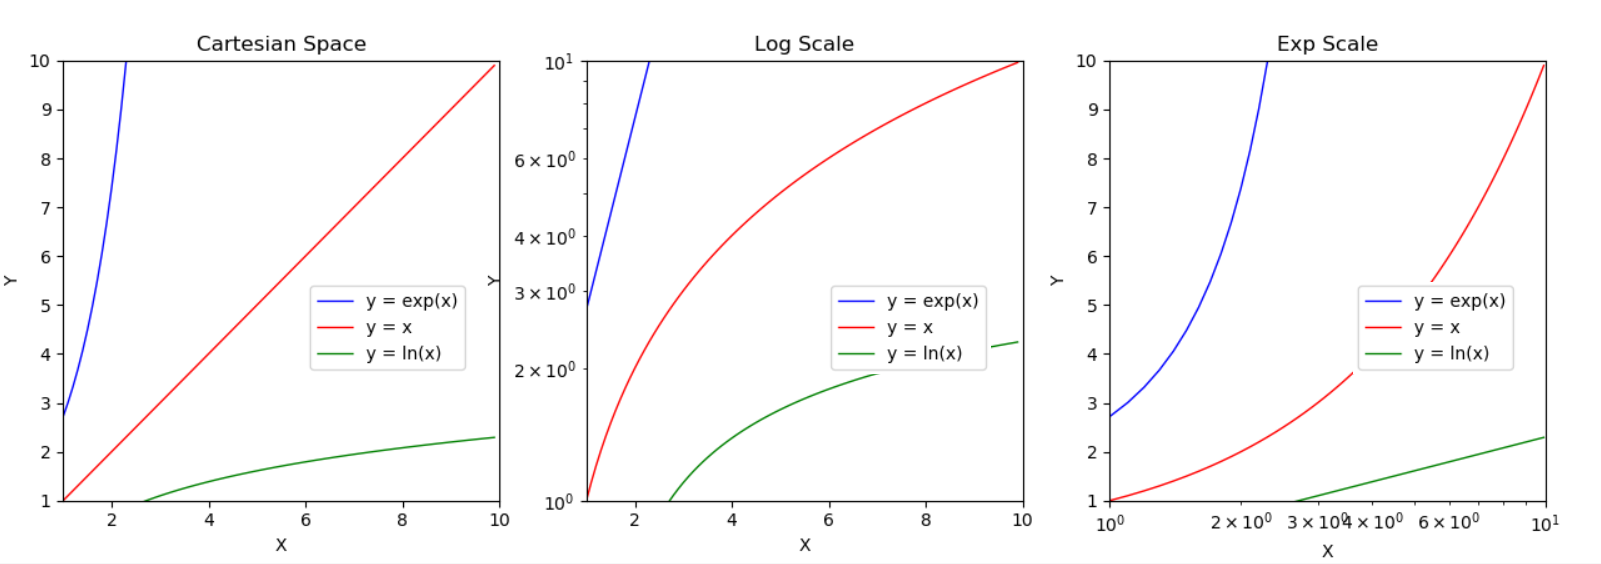
\includegraphics[scale=0.4]{Figures/diff_space.png}
    \par \textbf {Hình 1.1} Đồ thị hàm số trong các miền không gian khác nhau.
\end{center}
Đồ thị của hàm số $y=x$ trong miền không gian Cartesian có dạng đường thẳng, nhưng trong miền không gian mũ lại có dạng đường cong parabol, hoặc đồ thị hàm số $y=e^x$ có dạng parabol trong không gian Cartesian thông thường lại có dạng đường thẳng trong không gian logarit tự nhiên. Giá trị, số lượng các thông tin vẫn được bảo tồn và có thể thực hiện biến đổi qua lại giữa các miền không gian. Như vậy, việc khai thác đặc trưng các tín hiệu trong đa dạng các miền không gian sẽ mang lại những hiệu quả nhất định.
\par Có nhiều phép biến đổi tín hiệu sang các miền không gian khác nhau như biến đổi Cosine, biến đổi Fourier, biến đổi Wavelet,... Trong đó, biến đổi Fourier, thực hiện biến đổi tín hiệu từ miền thời gian sang miền tần số đóng vai trò rất quan trọng.
\section{Chuỗi Fourier và biến đổi Fourier}
\par Chuỗi Fourier (Fourier series) được nhà toán học người Pháp tên Jean Baptiste Joseph Fourier đưa ra vào đầu thế kỉ 19. Ông khẳng định rằng với bất kì hàm số $f(t)$ tuần hoàn với chu kì $T$ đều có thể biểu diễn được dưới dạng tổng của các hàm số sine và cosine với những tần số khác nhau, mỗi hàm số nhân với một hệ số tương ứng. Khi đó, ta gọi tổng các chuỗi hàm số sine và cosine này là chuỗi Fourier và quá trình biến đổi này được gọi là biến đổi Fourier. \\
\begin{center}
    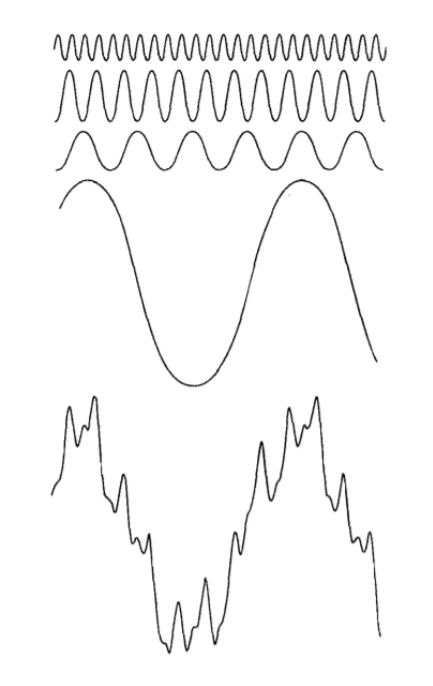
\includegraphics[scale=0.4]{Figures/fourier_example.png}
    \par \textbf {Hình 1.2} Ví dụ về chuỗi Fourier, hàm sóng cuối cùng là tổ hợp tuyến tính của các hàm sóng phía trên. 
\end{center}
Chuỗi Fourier của hàm tuần hoàn $p(t)$ có chu kì $T$ là:
\begin{equation}
  p(t) = \sum\limits_{n =  - \infty }^{ + \infty } {{c_n}{e^{j\frac{{2\pi n}}{T}t}}}. \tag{1.2-1}  
\end{equation}
Ta có công thức Euler trong trường số phức:
\begin{equation}
{e^{j\theta }} = \cos \theta  + i\sin \theta. \tag{1.2-2}
\end{equation}
Như vậy viết lại (1.2-1) ta được:
$$p(t) = \sum\limits_{n =  - \infty }^{ + \infty } {{c_n}(\cos (\frac{{2\pi n}}{T}t) + j\sin (\frac{{2\pi n}}{T}t))}.$$
\\
Trong đó:
\par $w=2\pi f=\frac{2\pi}{T}$
\par $w$ là tần số góc,
\par $f$ là tần số,
\par $T$ là chu kì,
\par $j$ là biến phức.

\subsection{Biến đổi Fourier cho hàm liên tục}
\subsubsection{Hàm một biến số}
Biến đổi Fourier thực chất là dạng biến đổi tổng quát từ khái niệm chuỗi Fourier.
Biến đổi Fourier của một hàm số liên tục $p(t)$, kí hiệu là $\mathcal{F} \{p(t)\}$ có công thức như sau:
\begin{equation}
\mathcal{F} \{p(t)\} = 
F(w ) = \int\limits_{ - \infty }^{ + \infty } {p(t){e^{ - jwt}}dt}.\tag{1.2-3}
\end{equation}
Ngược lại, cho trước hàm $F(w)$, ta có thể tìm lại hàm $p(t)$ bằng cách sử dụng biến đổi Fourier ngược (Inverse Fourier Transform):
\begin{equation}
\mathcal{F} ^{-1}\{F(w)\} = p(t) = \frac{1}{2\pi}\int\limits_{ - \infty }^{ + \infty } {F(w){e^{jwt}}dw} .\tag{1.2-4}
\end{equation}
Chứng minh:
Áp dụng công thức (1.2-3) cho vế phải, ta được:
\begin{equation*}
	\begin{split}
    VP & = \frac{1}{2\pi}\int\limits_{ - \infty }^{ + \infty } {F(w){e^{jwt}}dw} = \frac{1}{{2\pi }}\int\limits_{ - \infty }^{ + \infty } {(\int\limits_{ - \infty }^{ + \infty } {p(s){e^{ - jws}}ds){e^{jwt}}dw } } \\
    & = \frac{1}{{2\pi }}\int\limits_{ - \infty }^{ + \infty } {ds\,p(s)\,\int\limits_{ - \infty }^{ + \infty } {dw\,{e^{jw(t - s)}}} } \\
    & =\frac{1}{{2\pi }}\mathop {\lim }\limits_{N \to  + \infty } \int\limits_{ - \infty }^{ + \infty } {ds\,p(s)\,\frac{{{e^{j(t - s)N}} - {e^{ - j(t - s)N}}}}{{j(t - s)}}}.
	\end{split}
\end{equation*}

Áp dụng hệ quả công thức Euler (1.2-2):
$$VP=\frac{1}{{\pi }}\mathop {\lim }\limits_{N \to  + \infty } \int\limits_{ - \infty }^{ + \infty } {ds\,p(s)\,\frac{{\sin (N(t - s))}}{{t - s}}}
$$
Áp dụng shifting-property [3]:
\begin{equation*}
	\begin{split}
	VP &= \frac{1}{\pi }p(t)\mathop {\lim }\limits_{N \to  + \infty } \int\limits_{ - \infty }^{ + \infty } {ds} \frac{{\sin (N(t - s))}}{{t - s}} \\
	& = \frac{1}{\pi }p(t)\int\limits_{ - \infty }^{ + \infty } {dy} \frac{{\sin y}}{y} = p(t).
	\end{split}
\end{equation*}

Như vậy, ta được điều phải chứng minh.\\
\\
\textbf{Điều kiện áp dụng biến đổi Fourier}
\begin{itemize}
    \item $p(t)$ khả tích tuyệt đối
    $$\int\limits_{ - \infty }^{ + \infty } {|p(t)|dt < } \,\,\infty
.$$
    \item Trong một khoảng hữu hạn của $t$, $p(t)$ có hữu hạn cực đại và cực tiểu.
    \item Trong một khoảng hữu hạn của $t$, $p(t)$ có hữu hạn các điểm không liên tục và giá trị không liên tục là hữu hạn.
\end{itemize}

Ví dụ:
$$p(t) = \left\{ {\begin{array}{*{20}{c}}
{{e^{ - at}}\,\,\,\,(t > 0)}\\
{0\,\,\,\,(t < 0)}
\end{array}} \right.\,\,\,\,\,\,\,\,\,,\,a > 0.$$
Sử dụng định nghĩa (1.2-3), biến đổi Fourier của hàm số $p(t)$ trên là:
$$F(w) = \int\limits_{ - \infty }^{ + \infty } {p(t){e^{ - jwt}}dt = \int\limits_0^{ + \infty } {{e^{ - (a + jw)t}}dt = \frac{1}{{a + jw}}} } .$$
\subsubsection{Hàm hai biến số}
Với hàm hai biến số, ta có công thức biến đổi Fourier như sau:
\begin{equation}
\mathcal{F} \{p(x, y)\} = F(u,v) = \int\limits_{ - \infty }^{ + \infty } {\int\limits_{ - \infty }^{ + \infty } {p(x,y){e^{ - j({\rm{ux}} + vy)}}dx\,dy} }.\tag{1.2-5}
\end{equation}
Công thức biến đổi Fourier ngược
\begin{equation}
\mathcal{F}^{-1} \{F(u, v)\} = p(x,y) = \frac{1}{{4{\pi ^2}}}\int\limits_{ - \infty }^{ + \infty } {\int\limits_{ - \infty }^{ + \infty } {F(u,v){e^{j({\rm{ux}} + vy)}}dx\,dy} } .\tag{1.2-6}
\end{equation}
\subsection{Biến đổi Fourier cho hàm rời rạc}
\subsubsection{Hàm một biến số}
Với dãy $\{x_n\}$, $n=0, 1, 2,... N-1$ ta xây dựng DFT cho $x_n$ như sau 
\begin{equation}
\mathcal{F} \{x_n\} = {X_k} = \sum\limits_{n = 0}^{N-1} {{x_n}{e^{ - j\frac{{2\pi n}}{N}k}}} .\tag{1.2-7}
\end{equation}
Công thức IDFT
\begin{equation}
\mathcal{F}^{-1}\{X_k\} = {x_k} = \frac{1}{N}\sum\limits_{n = 0}^{N-1} {{X_n}{e^{j\frac{{2\pi n}}{N}k}}} .\tag{1.2-8}
\end{equation}
Chứng minh:
Từ định nghĩa DFT (1.2-7), ta có:
$$\frac{1}{N}\sum\limits_{n = 0}^{N-1} {{X_n}{e^{j\frac{{2\pi n}}{N}k}}} = \frac{1}{N}\sum\limits_{n = 0}^{N-1} {{
(\sum\limits_{m = 0}^{N-1} {{x_m}{e^{ - j\frac{{2\pi m}}{N}n}}})
}{e^{j\frac{{2\pi n}}{N}k}}} $$
$$=\frac{1}{N}\sum\limits_{m = 0}^{N-1} {{x_m}\sum\limits_{n = 0}^{N-1} {{e^{j\frac{{2\pi (k - m)}}{N}n}}} }
.$$
Nếu $k=m$ thì $\sum\limits_{n = 0}^{N-1} {{e^{j\frac{{2\pi (k - m)}}{N}n}}}=N.$\\
Nếu $k\neq m$ thì áp dụng công thức cấp số nhân, ta được:
$$S = \sum\limits_{n = 0}^{N-1} {{e^{j\frac{{2\pi (k - m)}}{N}n}}}
= \frac{{1 - {e^{j\frac{{2\pi (k - m)}}{N}N}}}}{{1 - {e^{j\frac{{2\pi (k - m)}}{N}}}}} = \frac{{1 - {e^{j2\pi (k-m)}}}}{{1 - {e^{j\frac{{2\pi (k - m)}}{N}}}}}.$$
Áp dụng công thức Euler (1.2-2):
$${e^{j2\pi (k - m)}} = \cos (2\pi (k - m)) + i\sin (2\pi (k - m)) = 1 $$
và
$${e^{\frac{{^{j2\pi (k - m)}}}{N}}} \ne 1 .$$
Do đó $S=0$ khi $k\neq m$, như vậy ta có điều phải chứng minh
$$\frac{1}{N}\sum\limits_{n = 0}^{N-1} {{X_n}{e^{j\frac{{2\pi n}}{N}k}}}= \frac{1}{N}x_k N = x_k.$$
\subsubsection{Hàm hai biến số}
Tương tự, ta có khai triển DFT cho hàm hai biến số
\begin{equation}
\mathcal{F} \{p(x,y)\} = F(u,v) = \frac{1}{{MN}}\sum\limits_{x = 0}^{M - 1} {\sum\limits_{y = 0}^{N - 1} {p(x,y){e^{ - j2\pi (\frac{{ux}}{M} + \frac{{vy}}{N})}}} } .\tag{1.2-9}
\end{equation}
Khai triển IDFT
\begin{equation}
\mathcal{F}^{-1} \{F(u,v)\}
p(x,y) = \sum\limits_{x = 0}^{M - 1} {\sum\limits_{y = 0}^{N - 1} {F(u,v){e^{j2\pi (\frac{{ux}}{M} + \frac{{vy}}{N})}}} }.\tag{1.2-10}
\end{equation}
\subsection{Tính chất}
Ta có một số tính chất cơ bản của phép biến đổi Fourier như sau:
\begin{itemize}
\item \textbf{Tính tuyến tính}
\par Nếu $F_1(w)\leftrightarrow p_1(t)$ và $F_2(w)\leftrightarrow p_2(t)$ \par thì $a_1 F_1(w) + a_2 F_2(w) \leftrightarrow a_1 f_1(t) + a_2 f_2(t) $, $a_1$, $a_2$ là các hằng số.


\item \textbf{Tính đối xứng (đối ngẫu thời gian - tần số)}
\par $p(t)\leftrightarrow F(w) \rightarrow F(t) \leftrightarrow 2\pi p(-w).$

\item \textbf{Tính đồng dạng}
\par $p(at)\leftrightarrow \frac{1}{|a|}F(\frac{w}{a}).$

\item \textbf{Tính dịch chuyển trong miền thời gian}
\par $p(t-t_0)\leftrightarrow {e^{ - jw{t_0}}}F(w).$

\item \textbf{Tính dịch chuyển trong miền tần số}
\par $p(t){e^{jw{t_0}}} \leftrightarrow F(w-w_0).$
\end{itemize}

\subsection{Thuật toán FFT (Fast Fourier Transform)}
Để biến đổi ảnh từ miền không gian sang miền tần số bằng cách sử dụng chuyển đổi Fourier rời rạc hai chiều thông thường đòi hỏi chi phí tính toán lớn khi kích thước ảnh lớn là $O(MN)$, hay đơn giản là $O(N^2)$ với $M,N$ là kích thước ảnh. Thuật toán FFT thực hiện giảm thiểu chi phí tính toán xuống $O(Nlog_2 N)$.
\par Thuật toán FFT thông dụng nhất là thuật toán do J.W.Cooley và John Tukey [4] đề xuất, biến đổi Fourier cho các giá trị rời rạc bằng cách sử dụng đệ quy tính các giá trị ở vị trí chẵn và lẻ. 
\subsubsection{FFT một chiều} 
\begin{align}
	{X_k} & = \sum\limits_{m = 0}^{\frac{N}{2}-1} {{x_{2m}}{e^{ - \frac{{j2\pi (2m)}}{N}k}}}  + \sum\limits_{m = 0}^{\frac{N}{2}-1} {{x_{2m + 1}}{e^{ - \frac{{j2\pi (2m + 1)}}{N}k}}} \notag \\
	& = \sum\limits_{m = 0}^{\frac{N}{2}-1} {{x_{2m}}{e^{ - \frac{{j2\pi m}}{{N/2}}k}}}  + {e^{ - \frac{{2\pi j}}{N}k}}\sum\limits_{m = 0}^{\frac{N}{2}-1} {{x_{2m + 1}}{e^{ - \frac{{j2\pi m}}{N/2}k}}} \notag \\
	& = E_k + {e^{ - \frac{{2\pi j}}{N}k}}O_k \tag{1.2-11}
\end{align}

với $E_k$ là DFT phần chẵn và $O_k$ là DFT phần lẻ. \\
Do tính tuần hoàn có chu kì nên
$E_{k+\frac{N}{2}}=E_k$
và
$O_{k+\frac{N}{2}}=O_k.$ \\
Khi đó, ta viết lại phương trình (1.2-11) thành
\begin{equation}
{X_k} = \left\{ {\begin{array}{*{20}{c}}
{{E_k} + {e^{ - \frac{{2\pi j}}{N}k}}{O_k}\,\,\,\,\,\,\,\,\,\,\,\,\,\,\,\,\,\,\,\,\,\,\,\,\,\,\,,\,0 \le k < \frac{N}{2}}\\
{{E_{k - N/2}} + {e^{ - \frac{{2\pi j}}{N}k}}{O_{k - N/2}}\,\,\,\,\,\,\,\,\,\,,\,\frac{N}{2} \le k < N.}
\end{array}} \right. \tag{1.2-12}
\end{equation} \\
Mặt khác, ta có
$${e^{ - \frac{{2\pi j}}{N}(k + N/2)}} = {e^{ - \frac{{2\pi j}}{N}k - \pi j}} =  - {e^{ - \frac{{2\pi j}}{N}k}}.$$ \\
Như vậy, ta có thể giảm khối lượng tính toán xuống một nửa. Với $0\le K < \frac{N}{2}$, từ phương trình (1.12-12) ta thu được:
$${X_k} = {E_k} + {e^{ - \frac{{2\pi j}}{N}k}}{O_k}
$$
$${X_{k + N/2}} = {E_k} - {e^{ - \frac{{2\pi j}}{N}k}}{O_k}.
$$

\par Tính DFT cho tín hiệu rời rạc 1 chiều có $2^n$ phần tử cẩn tới $(2^n)^2$ phép nhân. Tuy nhiên áp dụng FFT chỉ cần $n^{2^n}$. Do đó, về cơ bản tốc độ tính toán nhanh hơn $\frac{2^n}{n}$ lần.\\
\begin{center}
\begin{tabular}{|l|l|l|l|}
\hline
\multicolumn{1}{|c|}{\multirow{2}{*}{Kích thước}} & \multicolumn{2}{c|}{Số phép nhân} & \multicolumn{1}{c|}{\multirow{2}{*}{Tỉ lệ}} \\ \cline{2-3}
\multicolumn{1}{|c|}{}                            & Định nghĩa         & FFT          & \multicolumn{1}{c|}{}                                          \\ \hline
4                                                 & 16                 & 8            & 2.0                                                            \\ \hline
8                                                 & 84                 & 24           & 2.7                                                            \\ \hline
16                                                & 256                & 64           & 4.0                                                            \\ \hline
32                                                & 1024               & 160          & 6.4                                                            \\ \hline
64                                                & 4096               & 384          & 10.7                                                           \\ \hline
128                                               & 16384              & 896          & 18.3                                                           \\ \hline
256                                               & 65536              & 2048         & 32.0                                                           \\ \hline
512                                               & 262144             & 4608         & 56.0                                                           \\ \hline
1024                                              & 1048576            & 10240        & 102.4                                                          \\ \hline
\end{tabular}
\\
\end{center}
\begin{center}
    \textbf{Bảng 1.1:} So sánh thực hiện DFT theo định nghĩa và sử dụng FFT.
\end{center}

\begin{algorithm}[H]
	\SetAlgoLined
	\textbf{Input: }chuỗi số x, số lượng N, giá trị s.\\
	\textbf{Output: }chuỗi X = [X[0], X[1], ... X[N-1]].\\
	\textbf{function } X[0]...X[N-1] $\leftarrow$ $dfft$(x, N, s):\\
	\hspace{10mm} if N == 1 then \\
	\hspace{20mm} X[0] $\leftarrow$ x[0]\\
	\hspace{10mm} else\\
	\hspace{20mm} \# DFT cho X[0], X[2*s], X[3*s]...\\
	\hspace{20mm} X[0]...X[N/2-1] $\leftarrow$ $dfft$(x, N/2, 2s)\\
	\hspace{20mm} \# DFT cho X[s], X[3*s], X[5*s]...\\
	\hspace{20mm} X[N/2]...X[N-1] $\leftarrow$ $dfft$(x+s, N/2, 2s)\\
	\hspace{20mm} \# Kết hợp 2 nửa DFT thành 1 DFT\\
	\hspace{20mm} for k = 0 to N/2-1\\
	\hspace{30mm} t $\leftarrow$ X[k]\\
	\hspace{30mm} X[k] $\leftarrow$ t + exp(-2*PI*j*k/N)*X[k+N/2]\\
	\hspace{30mm} X[k+N/2] $\leftarrow$ t - exp(-2*PI*j*k/N)*X[k+N/2]\\
	\hspace{20mm} endfor\\
	\hspace{10mm} endif\\
	\caption{Thuật toán FFT - Fast Fourier Transform}
\end{algorithm}

\subsubsection{FFT hai chiều}
\par Ta có biến đổi dựa trên phương trình (1.2-9):
\begin{align*}
	\mathcal{F} \{p(x,y)\} & = F(u,v) = \frac{1}{{MN}}\sum\limits_{x = 0}^{M - 1} {\sum\limits_{y = 0}^{N - 1} {p(x,y){e^{ - j2\pi (\frac{{ux}}{M} + \frac{{vy}}{N})}}} } \\
	& = \frac{1}{M}\sum\limits_{x = 0}^{M - 1} {{e^{ - j2\pi \frac{{{\rm{ux}}}}{M}}}} \left[ {\frac{1}{N}\sum\limits_{y = 0}^{N - 1} {p(x,y){e^{ - j2\pi \frac{{vy}}{N}}}} } \right].
\end{align*}
Như vậy, biến đổi FFT hai chiều có thể được thực hiện bằng cách áp dụng biến đổi FFT một chiều trên từng hàng, sau đó biến đổi FFT trên từng cột.
\subsection{Định lý tích chập}
Cho hai hàm số liên tục $g(t)$ và $h(t)$, tích chập $*$ của hai hàm số này là
$$g(t)*h(t) = \int\limits_{ - \infty }^{ + \infty } {g(\tau )h(t - \tau )} d\tau .
$$
Áp dụng biến đổi Fourier sau khi sử dụng tích chập
$$\mathcal{F} \{g(t) * h(t)\} = \int\limits_{- \infty }^{ + \infty } \left[ \int\limits_{- \infty}^{+ \infty } g(\tau )h(t - \tau )d\tau  \right] e^{-jwt} dt.$$
Bằng phép đổi thứ tự lấy tích phân, ta được:
$$\mathcal{F} \{g(t) * h(t)\} = \int\limits_{ - \infty }^{ + \infty } {g(\tau ) \left[ \int\limits_{ - \infty }^{ + \infty } {h(t - \tau ) e^{-jwt}} dt \right] d\tau }.$$
Thực hiện phép đổi biến số $x=t-\tau$, ta được:
\begin{align*}
	\mathcal{F} \{g(t) * h(t)\} & =  \int\limits_{ - \infty }^{ + \infty } {g(\tau ) \left[ \int\limits_{ - \infty }^{ + \infty } {h(x) e^{ - j w(x + \tau ) } dx} \right] d\tau } \\
	& = \int\limits_{ - \infty }^{ + \infty } g(\tau ) \left[ \int\limits_{ - \infty }^{ + \infty } h(x)e^{ - jwx} dx \right] {{e}^{ - j w \tau }} d \tau \\
	& = H(w) \int\limits_{ - \infty }^{ + \infty } g(\tau ) { e^{ - jw \tau }}d\tau \\
	& = H(w)G(w),
\end{align*}

với $H(w)$, $G(w)$ là biến đổi Fourier của $h(t)$, $g(t)$.\\
Như vậy ta có:
$$\mathcal{F} \{g(t) * h(t)\} = H(w)G(w).$$
Định lý tích chập cho ta biết mối quan hệ giữa miền không gian và miền tần số, cụ thể, thông qua tích chập, một ảnh trong miền không gian có thể chuyển qua miền tần số và ngược lại. Phép tích chập được sử dụng trong miền không gian có thể được đơn giản hóa bằng phép nhân trong miền tần số thông qua biến đổi Fourier, thông qua đó tối thiểu hóa được chi phí tính toán. 
\section{Biến đổi Fourier trong xử lý ảnh số}
Biến đổi Fourier được sử dụng trong xử lý ảnh số chủ yếu là biến đổi Fourier rời rạc, vì mỗi bức ảnh được mã hóa dưới dạng ma trận hai chiều (đối với ảnh xám) và ba chiều (đối với ảnh màu thông thường như RGB, LAB, HSV,...). Đối với ảnh xám, mỗi điểm ảnh có giá trị từ 0 đến 255 biểu diễn cường độ ảnh. Do đó cường độ của điểm ảnh là một hàm số theo tọa độ trục tung và trục hoành tương ứng với vị trí của điểm ảnh đó.
\par Trong miền không gian, ta xử lý trực tiếp trên từng điểm ảnh, còn trong miền tần số, ta xử lý dựa trên tốc độ thay đổi giá trị trên miền không gian. Miền tần số có thể tạo ra mối quan hệ chu kỳ rõ ràng, giúp cho một số toán tử xử lý ảnh trở nên hiệu quả hơn, hoặc được đơn giản hóa chi phí tính toán. Do vậy, phép biến đổi Fourier đã được ứng dụng như một công cụ hữu hiệu để giải quyết các bài toán liên quan đến xử lý ảnh số.
\par Đối với bài toán phân đoạn ảnh (image segmentation), Paquet (1993)[17] giới thiệu cách tiếp cận mới để phân chia các mặt phẳng và tứ giác của hình ảnh 3D thông qua việc sử dụng biến đổi Fourier lên ảnh pha. Li và Wilson (1995)[12] đã xây dựng biến đổi Fourier đa phân giải (Multi Resolution Fourier Transform) để tiếp cận phân đoạn hình ảnh dựa trên phân tích thông tin địa phương trong miền không gian. Wu (1996)[23] đã trình bày thuật toán phân đoạn hình ảnh tế bào lặp bằng cách sử dụng các vectơ cường độ biến đổi Fourier thời gian ngắn như một đặc trưng của các lớp. Escofet (2001)[7] áp dụng biến đổi Fourier để phân đoạn hình ảnh và nhận dạng mẫu. Jianghong Li (2009)[13] sử dụng biến đổi Fourier trong việc phân đoạn các họa tiết động, nhằm xử lý chuỗi các hình ảnh thay đổi liên tiếp theo thời gian và không gian. 
\par Đối với bài toán phân loại hình ảnh (image classification), Grandlund (1972)[8] lần đầu tiên sử dụng biến đổi Fourier như một bước tiền xử lý trong việc nhận dạng ảnh kí tự viết tay. Robert (1980)[19] đã giới thiệu kĩ thuật phân loại hình ảnh vệ tinh tự động mà trong đó biến đổi Fourier rời rạc (DFT) được thiết kế để phát hiện và xác định tính năng của các đám mây từ mẫu hình ảnh chụp thường và hồng ngoại. Levchenko (1992)[11] đã thiết kết mô hình mạng nơron để phân loại hình ảnh đã được biến đổi Fourier. Harte và Hanka (1997)[9] đã xây dựng thuật toán cho vấn đề phân loại hình ảnh với kích thước lớn sử dụng biến đổi Fourier nhanh (FFT). Thông qua đó giải quyết được vấn đề về khối lượng tính toán đối với dữ liệu nhiều chiều. Tang và Stewart (2000)[21] sử dụng biến đổi Fourier để phân loại hình ảnh quang học. Hiệu suất phân loại của biến đổi Fourier được so sánh với biến đổi wavelet. Li-Wei Yang (2012)[14] sử dụng FFT trong nhận diện lá cây. Sokołowski (2014)[1] sử dụng trong phân loại ảnh nhận diện khối u ác tính. Popa (2018)[5] sử dụng FFT kết hợp với Complex-value Convolution Neural Network (CVCNNs) trong phân loại hình ảnh để tận dụng cả phần thực và phần ảo sau biến đổi, chỉ ra sự cải thiện độ chính xác so với chỉ sử dụng CNN trên trường số thực.
\par Biến đổi Fourier còn được sử dụng trong việc tái kết cấu ảnh (image reconstruction) như Matt Pharr (2004)[10] sử dụng thuật toán FFT trong việc tái kết cấu ảnh y tế, hay Rowe (2007)[6] sử dụng biến đổi Fourier để tái tạo tín hiệu và nhiễu của dữ liệu fMRI sử dụng thông tin của các ảnh pha sau biến đổi Fourier.
\par Trong những năm gần đây, với sự phát triển nhanh chóng của các ngành 4.0 như khoa học dữ liệu, trí tuệ nhân tạo, dữ liệu lớn,... biến đổi Fourier sử dụng trong xử lý ảnh số trong các thao tác tiền xử lý như lọc nhiễu, giảm mờ, sinh dữ liệu, trích chọn đặc trưng thô,... nhằm phục vụ cho mô hình mạng nơron học sâu. Trong khuôn khổ nội dung tiếp theo của đồ án sẽ trình bày về một số phương pháp tiền xử lý dữ liệu hình ảnh thông dụng và phương pháp trích chọn đặc trưng dựa trên biến đổi Fourier để xử lý bài toán nhận dạng mẫu.
%\begin{itemize}
%    \item Nén ảnh (ví dụ như chuẩn ảnh JPEG)
%item Lọc ảnh
%    \item Giảm mờ, nhiễu ảnh
%\end{itemize}
%Ngoài ra biến đổi Fourier còn được sử dụng nhưng một phương pháp %trích chọn đặc trưng sử dụng trong các mô hình nhận dạng như nhận %dạng khuôn mặt, nhận dạng kí tự viết tay



